
\documentclass[12pt,a4paper]{article}
\usepackage{times}
\usepackage{durhampaper}
\usepackage{harvard}
\usepackage{graphicx}

\citationmode{abbr}
\bibliographystyle{agsm}

\title{Implementation and Analysis of an Elliptic Curve Cryptography System}
%\author{} % leave; your name goes into \student{}
\student{T. Butterfield}
\supervisor{M. Bordewich}
\degree{BSc Computer Science}

\date{\today}

\begin{document}

\maketitle

\begin{abstract}
Do not cite references in the abstract.

This section should not be longer than half of a page, and having no more than one or two sentences under each heading is advised.

\paragraph{Background} -
Diffie-Hellman, RSA, ...

\paragraph{Aims} -
The aim of this project was to create a working Elliptic Curve Cryptography system 
and to analyse that system in terms of security and efficiency. 

\paragraph{Method} -
Euclid's extended algorithm, point addition, point multiplication, ...

\paragraph{Results} -
Cannot discover information about private key, enables secure communication

\paragraph{Conclusions} -
Strength of ECC, smaller key size than RSA, much more suitable for mobile devices

\end{abstract}


\begin{keywords}
Elliptic Curve Cryptography (ECC), Elliptic Curve Diffie-Hellman (ECDH), Elliptic Curve Digital Signature Algorithm (ECDSA), 
Safe Curves, User Interface (UI)
\end{keywords}


\section{Introduction} \noindent
There were a total of nine objectives for this project, split equally into three sections: basic, intermediate, and advanced. 

The first basic objective was to create a basic working ECC system which computed the essential functions required. 
The second and third basic objectives were to create a client application that can conduct ECDH over a network connection, 
and to create a UI allowing a user to easily make use of the system and to decide what level of complexity is revealed to them. 

The intermediate objectives revolved around improving the functionality and security of the system, 
with the first objective being to add secure random private key generation to the system. 
The other intermediate objectives were to implement the ECDSA and to enable the exchange of secure signed files via the UI. 

The first advanced objective was to make improvements to the UI and to reveal the workings of the system. 
The penultimate objective was to analyse the code for efficiency, including how the time required scales with the curve and key size, 
making any necessary changes to the system to improve the efficiency. 
The final objective was to analyse the code for vulnerabilities, such as side-channel attacks, and to fix any such weaknesses. 


\section{Related Work} \noindent
Cryptography is the study of mathematical systems for solving two kinds of security problems: privacy and authentication \cite{1055638}. 
A privacy system prevents the extraction of information by unauthorised parties from messages transmitted over a public channel, assuring it is read only by the intended recipient. 
An authentication system prevents the unauthorised injection of messages into a public channel, assuring the legitimacy of the sender. 
Diffie \& Hellman \citeyear{1055638} proposed that it was possible to develop systems in which two parties communicating solely over a public channel and using only publicly known techniques could create a secure connection. 
This was the first public discovery of public-key cryptography.

Diffie and Hellman presented the concept of a public-key cryptosystem but not any practical implementation of such a system. 
So in 1978, Rivest, Shamir, and Adleman presented a new encryption method which did just that, it was the first public implementation of public-key cryptography. 
This method had the novel property that publicly revealing an encryption key did not thereby reveal the corresponding decryption key \cite{10.1145/359340.359342}. 
This is known as RSA public-key cryptography. 

Miller \citeyear{10.1007/3-540-39799-X_31} and Koblitz \citeyear{koblitz1987elliptic} discussed an analogue of the Diffie-Hellman key exchange protocol based on elliptic curves over finite fields which used the multiplicative group of a finite field. 
The advantage of this system was that it appeared to be immune from attacks of the style of \cite{10.1007/3-540-39799-X_31,4568001}. 
This was the invention of Elliptic Curve Cryptography. 

Whilst the \emph{Elliptic Curve Discrete Logarithm Problem} is difficult to solve on classical computers \cite{hankerson2003guide}, 
there is a gap between ECDLP difficulty and ECC security \cite{bernstein2013safecurves}. 
In 2010, it was discovered that Sony had made a basic and critical mistake in the implementation of their Elliptic Curve Cryptosystem. 
As discussed in section \ref{Signature Generation}, as part of the Signature Generation stage of the ECDSA, a random integer $k$ is generated and used, 
it is imperative that $k$ is truly random and not predictable in any way. 
However, Sony wrote their own software which used a constant number for each signature. 
This allowed the computation of their private key, from the public key, using simple algebra \cite{hotz2010console}.


\subsection{Safe Curves} \noindent \label{Safe Curves}
There are several different standards covering selection of curves for use in elliptic-curve cryptography, 
most recently NSA Suite B (2005) and ANSSI FRP256V1 (2011). 
Each of these standards tries to ensure that the ECDLP (finding a user's private key, given their public key) is difficult. 
Unfortunately, there is a gap between ECDLP difficulty and ECC security. 
None of these standards do a good job of ensuring ECC security, 
secure implementations of the standard curves are theoretically possible but very hard. 
There are many attacks that break real-world ECC without solving ECDLP \cite{bernstein2013safecurves}. 
MORE DETAIL ABOUT WHAT MAKES A CURVE SAFE/UNSAFE

In 2006, Daniel Bernstein designed a new high-security ECDH function which achieved record setting speeds (twice as fast as any other function), 
with several side benefits including state-of-the-art timing-attack protection. 
This function, known as Curve25519, is suitable for a wide variety of cryptographic applications. 
The Curve25519 function is $F_p$-restricted x-coordinate scalar multiplication on $E(F_{p^2})$, 
where $p$ is the prime number $2^{255} - 19$ and $E$ is the elliptic curve $y^2 = x^3 + 486662x^2 + x$ \cite{10.1007/11745853_14}.
Curve25519 is regarded as a safe curve, since it satisfies the basic parameter requirements, the ECDLP security requirements, 
and the ECC security requirements beyond ECDLP security \cite{bernstein2013safecurves}.

\subsection{Exhaustive Search} \noindent \label{Exhaustive Search}
The elliptic curve parameters for cryptographic schemes should be carefully chosen in order to resist all known attacks on the ECDLP. 
The most na\"{\i}ve algorithm for solving the ECDLP is exhaustive search whereby one computes the sequence of points $P,2P,3P,4P,...$ until $Q$ is encountered. 
The running time is approximately $n$ steps in the worst case and $n/2$ steps on average. 
Therefore, exhaustive search can be circumvented by selecting elliptic curve parameters with $n$ sufficiently large to represent an infeasible amount of computation (e.g., $n \geq 2^{80}$) \cite{hankerson2003guide}.

\subsection{Pohlig-Hellman and Pollard's rho algorithm} \noindent \label{Pohlig-Hellman and Pollard's rho algorithm}
The best general-purpose attack known on the ECDLP is the combination of the Pohlig-Hellman algorithm and Pollard's rho algorithm, 
which has a fully-exponential running time of $O( \sqrt p \,)$ where $p$ is the largest prime divisor of $n$. 
To resist this attack, the elliptic curve parameters should be chosen so that $n$ is divisible by a prime number $p$ sufficiently large 
so that $\sqrt p$ steps is an infeasible amount of computation (e.g., $p > 2^{160}$).
If, in addition, the elliptic curve parameters are carefully chosen to defeat all other known attacks (e.g. Isomorphism attacks), 
then the ECDLP is believed to be infeasible given the state of today's computer technology \cite{hankerson2003guide}.



\section{Solution} \noindent
This section presents the solutions to the problems in detail. 
Included here are details of the specification and design (Section \ref{Specification}), 
an outline of the implementation issues faced (Section \ref{Implementation}), 
as well as a description of the tools used (Section \ref{Tools}), 
and finally verification and validation of the components (Section \ref{Verification}). 

\subsection{Architecture and Design} \noindent \label{Specification}
At a high level, my system is a client-server network designed to allow 
multiple instances of a client program to connect to a single server program. 
The clients can communicate with each other, via the server, using end-to-end ECC encryption. 
In the description and explanation of my system I will personalise the participants; 
Alice and Bob want to communicate while Eve, the eavesdropper, intercepts and tries to read their messages. 
Figure \ref{fig:messages} illustrates the protocol for Alice to send a message to Bob: 

\begin{figure}[htb]
    \centering
    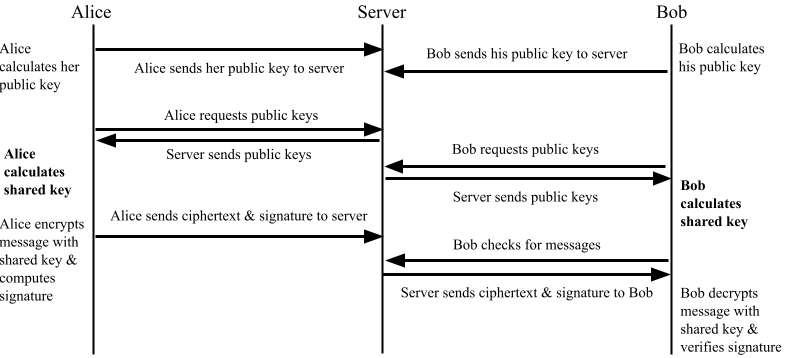
\includegraphics[width=\textwidth]{figures/Message Exchange Diagram.png}
    \caption{Message Exchange Diagram}
    \label{fig:messages}
\end{figure}

A message here can be either a text message or a file from Alice's device. 
The server stores a list of the public keys of every client who is connected, 
and will send this to any client who requests it in order for them to establish a shared key with other clients. 
The server also holds the encrypted data and the accompanying signature for messages which have yet to be requested by the recipient. 
After the recipient has asked the server if there are any messages waiting for them, the server has sent the relevant message(s), 
and the recipient has decrypted and verified the message(s), the server then deletes the message(s). 
The only data stored by the client is a list of their shared keys with other clients. 
As shown in Figure \ref{fig:messages}, all of the computation is done by the client and the server does not perform any calculations; 
it only receives, stores, and sends client data. 
There are two ECC specific algorithms performed by each client in the exchange shown in Figure \ref{fig:messages}, 
namely the Elliptic Curve Diffie-Hellman (ECDH) key exchange algorithm and the Elliptic Curve Digital Signature Algorithm (ECDSA). 

\subsection{Algorithms} \noindent \label{Algorithms}
This section outlines the algorithms which are used by my system and how I implemented them. 
The two ECC specific algorithms mentioned previously (ECDH and ECDSA) differ from their RSA counterparts (DH and DSA) only in that 
the operation of exponentiation of an integer is instead replaced by the operation of multiplying a point on an elliptic curve. 
The naive approach to this of repeatedly adding a point $G$ to itself $k$ times in order to calculate $kG$ would take prohibitively long. 
Therefore I had to implement an adapted version of the repeated squares method (squaring and multiplying integers) 
used by RSA to calculate large exponents efficiently. 
This adapted method I implement is to use doubling and adding of points on an elliptic curve in order to achieve multiplication of a point. 
While the naive approach would take $O(k)$ time to calculate $kG$, this approach takes $O(log(k))$ time, 
making it practical for my system since $k$ will be a very large number (of the order $2^{250}$). 
An elliptic curve (Section \ref{Elliptic Curve}), along with the operations of adding (Section \ref{Point Addition}) 
and doubling (Section \ref{Point Doubling}) points on the curve, are formally defined below. 

\subsubsection{Elliptic Curve} \noindent \label{Elliptic Curve}
Let $p$ be a prime number, and let $F_p$ denote the field of integers modulo $p$. 
An elliptic curve $E$ over $F_p$ is defined by an equation of the form:
\begin{equation}
y^2 = x^3 + ax + b,
\end{equation}

where $a,\, b \in F_p$ satisfy $4a^3 + 27b^2 \ne 0$ (mod $ p$).

\subsubsection{Point Addition} \noindent \label{Point Addition}
Let $P = (x_1,y_1) \in E(F_p)$ and $Q = (x_2,y_2) \in E(F_p)$, where $P \neq Q$. 
Then $P + Q = (x_3,y_3)$, where:
\begin{equation}
    x_3 = \lambda^2 - x_1 - x_2, \quad y_3 = \lambda(x_1 - x_3) - y_1, \quad and \quad \lambda = \frac{y_2-y_1}{x_2-x_1}.
\end{equation}

\subsubsection{Point Doubling} \noindent \label{Point Doubling}
Let $P = (x_1,y_1) \in E(F_p)$. 
Then $P + P = 2P = (x_3,y_3)$, where:
\begin{equation}
    x_3 = \lambda^2 - 2x_1, \quad y_3 = \lambda(x_1 - x_3) - y_1, \quad and \quad \lambda = \frac{3x_1^2 + a}{2y_1}
\end{equation}

\cite{hankerson2003guide,lopez2000overview}.

\vspace{5mm}

In my system when I want to multiply a point $G$ by an integer $k$, 
I take the point $G$ and double it $\lfloor log_2(k) \rfloor$ times, storing each new point in an array where index $i$ holds $2^i \cdot G$. 
The final value is then calculated by adding the points in the array whose index corresponds to a $1$ in the binary expansion of $k$. 
My system actually implements this using bitwise operations on $k$ for efficiency, 
however it is more intuitive to imagine it as a binary expansion and an array of equal length as described. 
That is how I implement point multiplication using point addition and point doubling. 
Things are complicated further however due to the fact that an elliptic curve is defined over a field of integers modulo $p$ (\ref{Elliptic Curve}), 
meaning that these operations are all carried out in modulo $p$ and can only involve integers. 
Since the equations for both point addition (\ref{Point Addition}) and point doubling (\ref{Point Doubling}) involve division, 
it is clear that a naive implementation of division cannot be used here since it would produce non-integer results. 
Therefore I had to implement the Extended Euclidean algorithm (EEA) in order to ensure integer results of these division calculations. 
For example, in order to calculate the gradient $\lambda = \frac{y_2-y_1}{x_2-x_1}$ in point addition (\ref{Point Addition}), 
I use the EEA to calculate $(x_2-x_1)^{-1}$ mod $p$ and then multiply this by $(y_2-y_1)$. 
This ensures that $\lambda$ is an integer, and therefore that the coordinates $(x_3,y_3)$ as defined in \ref{Point Addition} 
are also integers. 

Once I had a function for efficiently computing point multiplication, I was able to move on to the functions of ECDH and ECDSA. 

\subsubsection{ECDH} \noindent \label{ECDH}
The \emph{Elliptic Curve Diffie-Hellman} key agreement protocol allows Alice and Bob 
to securely agree upon the value of a point on an elliptic curve, although neither of them initially knows the value of the point. 
This point becomes their shared key, and the algorithm for generating it is formally defined below. 


\subsubsection{Shared Key Establishment} \noindent \label{SharedKey}
Alice and Bob must agree on a finite field $F_p$, an elliptic curve $E/F_p$, and a base point $G \in E(F_p)$  of (prime) order $n$.
Both Alice and Bob have a key pair $(d,Q)$ consisting of a private key $d$ (a randomly selected integer less than $n$) 
and a public key $Q = d * G$.

\vspace{1mm}

0. \space Let $(d_A,Q_A)$ be the key pair of Alice and $(d_B,Q_B)$ be the key pair of Bob.

1. \space Alice computes $K = (x_K,y_K) = d_A * Q_B$

2. \space Bob computes $L = (x_L,y_L) = d_B * Q_A$

3. \space Since $d_AQ_B = d_Ad_BG = d_Bd_AG = d_BQ_A$. Therefore $K = L$ and hence $x_K = x_L$

4. \space Hence the shared secret is $x_K$

\vspace{1mm}

Since it is practically impossible to find the private key $d_A$ or $d_B$ from the public key $K$ or $L$, 
it is not possible for Eve to obtain the shared secret \cite{jurivsic1997elliptic,anoop2007elliptic,silverman2009arithmetic,brown2009standards}. 

\vspace{5mm}

In my implementation of this algorithm, all clients are automatically using the same base point which lies 
on the same elliptic curve, defined over the same finite field. 
This is because every client is an instance of the same program and this is hard-coded. 
I generate the random private key for each client, using Python's "secrets" module, when the client instance is started. 
The public key is then calculated using the point multiplication function mentioned previously. 
This public key is sent to the server along with the user's name (e.g. Alice) which they have entered via the command line. 
Any other user (e.g. Bob) can then get Alice's public key from the server and establish a secret shared key with her. 
In my system, Bob (or any other client) calculates their shared key with Alice by first asking the server 
for any available public keys. 
Bob then uses the point multiplication function to multiply Alice's public key by his private key. 
The shared keys that each client has established with their contacts are stored locally 
and used to encrypt future messages with symmetric AES. 

\subsubsection{ECDSA} \noindent \label{ECDSA}
The \emph{Elliptic Curve Digital Signature Algorithm} allows Alice to sign a message or file in such a way that Bob is able to then 
verify that Alice must have been the sender and that the message/file has not been altered. 
Alice does this by generating a signature using the hash of the message and her private key. 
She then sends this to Bob alongside her message. 
Bob then uses Alice's public key and the hash of the message to check that the signature must have been generated on the same message and by Alice. 
The two parts of this algorithm are formally defined below. 

\subsubsection{Signature Generation} \noindent \label{Signature Generation}
For signing a message $m$ sent by Alice, using Alice's private key $d_A$.

\vspace{1mm}

1. \space Calculate $e = HASH(m)$, where $HASH$ is a cryptographic hash function, such as SHA

2. \space Select a random integer $k$ from $[1,n-1]$

3. \space Calculate $r = x1$, where $(x1,y1) = k * G$ (mod $n$)

4. \space Calculate $s = k^{-1}(e+d_Ar)$ (mod $n$)

5. \space The signature is the pair $(r,s)$

\subsubsection{Signature Verification} \noindent \label{Signature Verification}
For Bob to authenticate Alice's signature, Bob must have Alice's public key $Q_A$.

\vspace{1mm}

1. \space Calculate $e = HASH(m)$

2. \space Calculate $w = s^{-1}$ (mod $n$)

3. \space Calculate $u_1 = ew$ (mod $n$) and $u_2 = rw$ (mod $n$)

4. \space Calculate $(x_1,y_1) = u_1G + u_2Q_A$

5. \space The signature is valid if $x_1 = r$ (mod $n$), invalid otherwise

\vspace{2mm}

\cite{jurivsic1997elliptic,koblitz2000state,hankerson2003guide,anoop2007elliptic,silverman2009arithmetic,brown2009standards}.

\vspace{5mm}

In my implementation of this algorithm, Alice and Bob first agree upon all of the same initial setup things mentioned in Section \ref{ECDH} 
by default since again they are all hard-coded in to every client. 
When Alice wants to send a signed message or a file to Bob, she enters the message or the name of the file via the command line, 
and generates a hash of the message/file using SHA-512 from Python's "hashlib" module. 
This hash is converted to an integer and truncated to be smaller than $n$. 
A random number $k$ is then generated using the same "secrets" module previously mentioned and the point $G$ is multiplied by $k$ using 
the point multiplication function, with the x-coordinate taken as $r$ and the y-coordinate discarded. 
The integer $r$ is multiplied by Alice's private key (also an integer) and added to the truncated hash of the message (another integer), 
finally this is divided by $k$ to generate $s$. 
This division is done by multiplying by the inverse of $k$ modulo $n$, calculated with the EEA function mentioned earlier. 
Alice sends both $r$ and $s$ to the server, along with her AES encrypted message. 

On the receiving end of my implementation, after Bob receives all of this data from the server, 
he first decrypts the message itself using the shared key he has already established with Alice. 
He uses the plaintext message and the same hashing algorithm to generate a hash of the message, 
which he converts to an integer and truncates in the same way that Alice did, calling it $e$. 
The multiplicative inverse of $s$ modulo $n$ is then calculated using the EEA function and called $w$. 
Bob then does two integer multiplications, the first is the $e*w$ (mod $n$), 
and the second is $r*w$ (mod $n$), these new integers are called $u_1$ and $u_2$ respectively. 
Next, two lots of point multiplication are carried out and their results are summed by point addition. 
The first point multiplication is $u_1*G$ where $G$ is the base point mentioned previously, 
and the second is $u_2*Q_A$ where the point $Q_A$ is Alice's public key. 
After adding these two points together using the point addition function to create a new point, 
Bob takes just the x-coordinate of this new point and compares it to the $r$ from Alice's signature. 
If these are equal (mod $n$) then the signature is valid and was definitely generated by Alice using the same message which Bob received. 
So now Bob has the plaintext message and is assured that it is authentic. 


\subsection{Tools used} \noindent \label{Tools}
The system was created entirely in Python. 
I chose this language because of both its ability to handle large integers with ease, 
and its large number of well-established modules for computing generic cryptographic functions. 
Since my system carries out operations involving huge integers, other less abstracted languages would 
have required much more involvement at the lower level which would only detract from my progress with the actual aims of the project. 
The specific Python modules that I used in my system are: "Pyro4", "AES" from "Cryptodome", "base64", "hashlib", "secrets", and "os". 
"Pyro4" is used for remote object invocation, "AES" for symmetric encryption, "base64" for decoding the AES ciphertext, 
and "hashlib" for generating hashes using SHA-2. 
I chose to use "secrets" because I realised that my initial implementation using "random" was not cryptographically secure. 
I used the "os" module for file management, since any files which the user receives are stored 
in a subdirectory labelled by their name. 
I only used long standing and well used libraries because of \cite{ducklin2021python}. 

The system can be started and interacted with via a command line interface. 
This was chosen since it allowed me to focus 
more on the protocols and back-end of the system rather than on designing a visually appealing graphical user interface (GUI). 
A GUI was not relevant to the mathematical-based aims of this project. 


\subsection{Implementation Issues} \noindent \label{Implementation}
After I successfully implemented client-client communication with separate instances of the client program running on the 
same machine, I then attempted to adapt the system for use with the client instances on separate machines on the same network. 
However, I encountered issues with this due to the security protocols in place on networks. 
I decided against attempting to circumvent these protocols due to both the potentially 
time-consuming nature of the problem and fact that my project is not aiming 
to recreate Signal or WhatsApp, network communication is not necessary. 


\subsection{Verification and Validation} \noindent \label{Verification}
This section will run through a real interaction between Alice and Bob using the system, 
specifically the exchange shown in Figure \ref{fig:messages}. 
This will demonstrate the calculations performed by the system and the validity of these calculations. 
All large numbers here are shown in hexadecimal, for brevity. 
This interaction uses an elliptic curve known as Curve25519 \cite{10.1007/11745853_14}, 
which can be expressed by the equation: 

\begin{equation}
    y^2 = x^3 + 486662x^2 + x \pmod{2^{255}-19}.
\end{equation}

This curve is most often expressed in the Montgomery \cite{montgomery1987speeding} form as above ($By^2 = x^3 + Ax^2 + x$), 
but can be converted to the more traditional short Weierstrass form shown earlier ($y^2 = x^3 + ax + b$) through substitution. 
Curve25519 has the base point $g = $ \\
({\footnotesize $0x9$}, {\footnotesize $0x20ae19a1b8a086b4e01edd2c7748d14c923d4d7e6d7c61b229e9c5a27eced3d9$}), \\
which has prime order $n = 2^{252} +$ {\footnotesize $0x14def9dea2f79cd65812631a5cf5d3ed$}. 
The curve's cofactor is $h = 8$. 


\subsubsection{Key Generation} \noindent
Alice's randomly generated private key is \\
{\footnotesize $0x69837a193b0f43bac8b32a30396a189c51706d49fcbb7c0e099b8f1b4bcb969$}. \\
When she multiplies the base point $g$ by this number, she obtains the point \\
({\footnotesize $0x67bf8995372ae1a9329f441d955193623aedf68a01ee5e2af7c33eabc27d9fd$}, \\
{\footnotesize $0xbc9a2fe41909056a46927d7c3af1ffed8e802854a32378df1845f819c016bdb$}) \\
as her public key.

Generated in the same way, Bob's private key is \\
{\footnotesize $0xf7d16d30314975879241ab2a17fdb1194fa2a7319b0b3331590c8482437f0b3$}. \\
Therefore his public key is \\
({\footnotesize $0x2ffeaa851900d44817e3888854d958a91b9e1127ed0057a2e6796f3a1115cda$}, \\
{\footnotesize $0x3fd4639dbd63076c19aeb51816711d7de4331cb75ec3c89ea1c387297660809c$}).


\subsubsection{Shared Key Establishment} \noindent
Alice calculates the shared key by $h \cdot d \cdot Q$, 
where $h$ is the cofactor, $d$ is Alice's private key, and $Q$ is Bob's public key. \\
Firstly, $d \cdot Q = $\\
({\footnotesize $0x7bb294204beba6ba902f5a21e14c4d5abc953d52b79be70377104f72de310a4a$}, \\
{\footnotesize $0x6d9d2ec13fc729a629259a1fcdf96d4a66e7e4e1365f54ed5fa56e235bc74b5$}) \\
Then multiplying by $h = 8$ gives $h \cdot d \cdot Q = $\\
({\footnotesize $0x37ae8d3aa1495b39ead29b8abe24e7d8d7f2fb05186216a37c4b55708ead1fd$}, \\
{\footnotesize $0x29aecf95ba814e3e52866f5daa243d3366e8c8d0255117ee047822319b44222c$}) \\
Therefore, Alice calculates the shared key as: 
\begin{equation} \label{AliceKey}
    0x37ae8d3aa1495b39ead29b8abe24e7d8d7f2fb05186216a37c4b55708ead1fd.
\end{equation}

Bob also calculates $h \cdot d \cdot Q$, except here $d$ is his private key and $Q$ is Alice's public key. 
$d \cdot Q = $ \\
({\footnotesize $0x7bb294204beba6ba902f5a21e14c4d5abc953d52b79be70377104f72de310a4a$}, \\
{\footnotesize $0x6d9d2ec13fc729a629259a1fcdf96d4a66e7e4e1365f54ed5fa56e235bc74b5$}) \\
Then multiplying by $h = 8$ gives $h \cdot d \cdot Q = $\\
({\footnotesize $0x37ae8d3aa1495b39ead29b8abe24e7d8d7f2fb05186216a37c4b55708ead1fd$}, \\
{\footnotesize $0x29aecf95ba814e3e52866f5daa243d3366e8c8d0255117ee047822319b44222c$}) \\
Bob's calculation of the shared key is: 
\begin{equation} \label{BobKey}
    0x37ae8d3aa1495b39ead29b8abe24e7d8d7f2fb05186216a37c4b55708ead1fd.
\end{equation}

This demonstrates that the ECDH part of the system works, since Alice and Bob each calculate the same shared key ( Key (\ref{AliceKey}) = Key (\ref{BobKey}) ). 
Critically, from a security perspective, only Alice and Bob can possibly know the value of this shared secret key 
because it was calculated using their respective private keys (which only they have access to). 
This makes it suitable for use as a symmetric AES key for end-to-end-encrypted communication between Alice and Bob. 


\subsubsection{Encryption} \noindent \label{Example1}
The system allows Alice to send a message or file to Bob which is encrypted using the shared key that they have just established (through ECDH). 
The following subsections (\ref{Example1}, \ref{Example2}, \ref{Example3}, \ref{Example4}) show an example message sent by Alice to Bob, 
as in Figure \ref{fig:messages}. 

\vspace{1mm}

Alice wants to send the message ``Hello, Bob!" to Bob. 
Their shared key is first converted from an integer to byte format, which is: \\
{\footnotesize $b' \char`\\x03z \char`\\xe8 \char`\\xd3 \char`\\xaa \char`\\x14 \char`\\x95 \char`\\xb3 \char`\\x9e \char`\\xad) \char`\\xb8 \char`\\xab \\ 
\char`\\xe2N\} \char`\\x8d \char`\\x7f/ \char`\\xb0Q \char`\\x86!j7 \char`\\xc4 \char`\\xb5W \char`\\x08 \char`\\xea \char`\\xd1 \char`\\xfd '$} \\
(in big-endian byte order). 

This is then hashed for security purposes, which generates the AES key: \\
{\footnotesize $b' \char`\\x00 \char`\\x0b \char`\\x0f \char`\\xe8 \char`\\xbfl \char`\\xa9 \char`\\xbb0 \char`\\x00(* \char`\\x92 \char`\\x01 \char`\\xba \char`\\xba \\ 
\char`\\xadU \char`\\xc2K8 \char`\\x08 \char`\\x1a \char`\\xdbL \char`\\xb8U \char`\\xcf \char`\\x15 \char`\\x94 \char`\\xcf \char`\\xca '$}. 

AES is used in EAX mode (encrypt-then-authenticate-then-translate) to generate the triple $(nonce, ciphertext, tag)$, where: 
\vspace{1mm} \\
$nonce = $ {\footnotesize $b' \char`\\xe0 \char`\\x80 \char`\\x00 \char`\\x8e \char`\\xd63rPd \char`\\xa3 \char`\\x161 \char`\\xe5l \char`\\xf0 \char`\\xe4 '$}, \\
$ciphertext = $ {\footnotesize $b' U \char`\\x15 \char`\\xe9 \char`\\x17 \char`\\xce4 \char`\\xa7 \char`\\xd9 \char`\\xbc: \char`\\xc6 '$}, \\
$tag = $ {\footnotesize $b' [V \char`\\xb2R \char`\\x85k \char`\\xb0UZRW \char`\\xf7? \char`\\xf8 \char`\\x14G'$}. 

\vspace{1mm}

This triple is then sent to Bob, along with the signature generated in \ref{Example2}. 


\subsubsection{Signature Generation} \noindent \label{Example2}
As mentioned, Alice can send an encrypted message to Bob, 
but she can also digitally sign it in such a way that Bob can verify the authenticity of the message. 
Here the signature is generated using the procedure outlined in Section \ref{Signature Generation}. 

The message (``Hello, Bob!") is hashed and then truncated to give the integer $e =$ \\
{\footnotesize $0x144b549f0522c7f6c224fe404e8200cfbe352c16883f16777d01ba8c81bce487$}. \\
Alice generates a random number $k$ and calculates $r = kG =$ 
\begin{equation} \label{AliceSig}
    0xa96542405f3dc83b44e45beaa40d911efe8c5fee82a9f087cce28882b0fca82.
\end{equation}
Next, she calculates $s = k^{-1}(e + d \cdot r) =$ \\
{\footnotesize $0x237543088442522d4dfb6acb7126982df6d73473d1d89fe0d26f24226d79e82$}, where $d$ is her private key. 

The signature that Alice sends, alongside the encrypted message triple, is the pair $(r,s)$. 
Therefore, in total, Alice sends the quintuple $(nonce, ciphertext, tag, r, s)$. 


\subsubsection{Decryption} \noindent \label{Example3}
Bob receives the quintuple $(nonce, ciphertext, tag, r, s)$. 
He uses the triple $(nonce, ciphertext, tag)$, along with his shared key, to decrypt the message. 
Bob converts the shared key from an integer to byte format, which he hashes to generate the same AES key as Alice did in Section \ref{Example1}. 
This AES key, along with the nonce, is used to decrypt the ciphertext. 
The plaintext is: "Hello, Bob!". 
The tag is also used to verify the authenticity of the message, 
although this is not strictly necessary since additional ECC authentication is done in Section \ref{Example4}. 


\subsubsection{Signature Verification} \noindent \label{Example4}
After decrypting the message with AES, Bob uses the signature pair $(r,s)$ to verify Alice's ECC signature 
using the procedure outlined in Section \ref{Signature Verification}. 
He first hashes the plaintext and truncates it to get the integer $e =$ \\
{\footnotesize$0x144b549f0522c7f6c224fe404e8200cfbe352c16883f16777d01ba8c81bce487$}. \\
Note that this is the same hash generated by Alice, but Bob doesn't yet know this since the hash itself is not sent. 
Alice calculates the x-coordinate of the point $v = (e \cdot s^{-1})G + (r \cdot s^{-1})Q =$ \\
\begin{equation} \label{BobSig}
    0xa96542405f3dc83b44e45beaa40d911efe8c5fee82a9f087cce28882b0fca82,
\end{equation}
where $Q$ is Alice's public key. 

Since this $v$ matches the $r$ in Alice's signature ($v=r$), 
Bob is assured that Alice sent the message, and that the content of the message is unchanged, 
since both Alice's private key, and the same hash must have been used to generate the signature. 

\vspace{5mm}

This demonstration both verifies and validates my system. 
The fact that both Alice and Bob calculate the same shared key, (\ref{AliceKey}) and (\ref{BobKey}), 
verifies and validates that the ECDH algorithm for key establishment has been implemented correctly in my system. 
While the fact that Alice's $r$ generated in (\ref{AliceSig}) matches Bob's $v$ generated in (\ref{BobSig}) 
verifies and validates that the ECDSA algorithm for both signature generation and verification has also been implemented correctly. 



\section{Results} \noindent \label{Results}
This section presents the results of various tests carried out on the system. 
These tests analyse both the efficiency (Section \ref{Efficiency}) and the security (Section \ref{Security}) of my system. 
In terms of efficiency, this includes a comparison between my ECC system and a standard RSA implementation, 
as well as a comparison between various ECC curves which my system can use. 
When analysing the security of my system, I look at whether any information about the private key is leaked through side-channel attacks, 
specifically timing attacks. 
All tests were carried out using a machine with an AMD Ryzen 5 3600 processor (3.6 GHz base, 4.2 GHz boost). 

\subsection{Efficiency} \noindent \label{Efficiency}
Perhaps the most significant claimed benefit of using ECC is its superior efficiency over RSA. 
Therefore I start here with a timing comparison between my ECC system and an RSA implementation 
from the ``PublicKey" package of the ``PyCryptodome" library. 
Specifically, the operation being timed here is the generation of a key pair, meaning both private and public key generation, 
of varying security strength. 
It is important to note that security strength is not the same as the key size, this is due to attacks on both RSA and ECC that provide computational advantages. 
As an example, a security strength of 112 bits requires an RSA key size of 2048 bits and an ECC key size of 224 bits \cite[p54-55]{barker2020recommendation}. 

For my ECC system I am measuring the time taken to both choose a random private key of the given security strength, 
and to then multiply the base point of the curve (M-511) by this number to create the corresponding public key. 
For RSA I am measuring the time taken to return a key pair of a specified security strength by the library function ``RSA.generate()". 
Figure \ref{fig:rsa} shows the results of this comparison for key pairs of 5 different security strengths (excluding 0). 
The top graph in Figure \ref{fig:rsa} shows the overall comparison, while the bottom graph shows the same results with a scaled y-axis. 

The most apparent finding of Figure \ref{fig:rsa} is that the time taken by my ECC system scales linearly as security strength increases, 
whereas the time taken by RSA scales exponentially. 
The second point to make about these results is that the bottom graph in Figure \ref{fig:rsa} shows RSA up to a security strength of 112 bits, 
which is today's minimum recommended level of security according to NIST \cite[p54-55]{barker2020recommendation}. 
Even at today's minimum security level RSA takes nearly an order of magnitude longer than ECC to generate a key pair (0.82s v 0.096s here). 
It is also important to consider that, due to the nature of computer advancement, this minimum security level will only increase over time. 
This means that the benefits of using ECC over RSA will only increase over time, 
for example when the recommended security level moves to 128 bits, the time difference will widen further. 
In these results that difference is 4.9 seconds for RSA against 0.11 seconds for ECC. 
In general this is the nature of comparing a $O(n^2)$ system with a $O(n)$ system. 
ECC is faster than RSA today, and will get even faster (relatively) in the future. 

% RSA = [0.8297,4.9126,96.7222,1024.2669]
% times511 = [0.0960,0.1100,0.1645,0.2221]

%also mention smaller key size means less data transfer and less computation for mobile devices

%When comparing the security strength of RSA with ECC it is important to bear in mind that for keys of the same length 
%RSA is faster than ECC, since the operation of multiplying integers is easier than adding points on an elliptic curve. 

%112 bit security strength, 2048 bits of RSA is equivalent to 224 bits of ECC
%128 bit security strength, 3072 bits of RSA is 256 bit ECC, this will be minimum requirement after 2023
%192, 7680, 384
%256, 15360, 512

%The measurement used to relate encryption algorithms to each other is the estimated maximum-security strength (in bits) 
%provided by the algorithm for a particular key length. 
%For example, according to NIST, to achieve a security strength of 112 bits, RSA requires a 2048 bit key, whereas ECC requires a 224 bit key. 
%this measurement takes into account attacks on the algorithms that provide computational advantages. 

\begin{figure}[!htb]
    \begin{minipage}{0.5\textwidth}
        \centering
        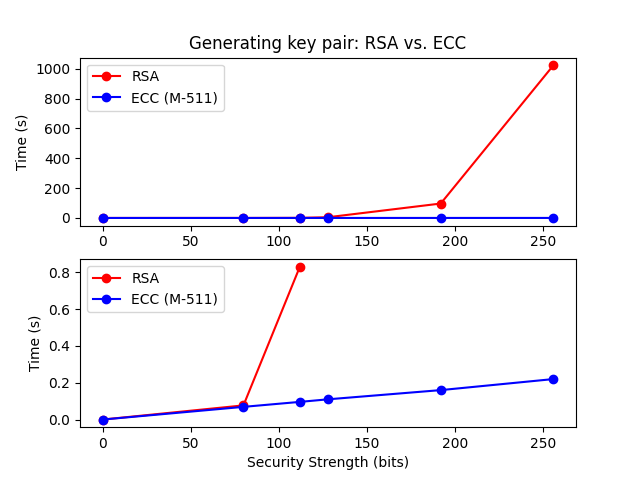
\includegraphics[width=\linewidth]{figures/RSA.png}
        \caption{ECC more efficient than RSA}
        \label{fig:rsa}
    \end{minipage}\hfill
    \begin{minipage}{0.5\textwidth}
        \centering
        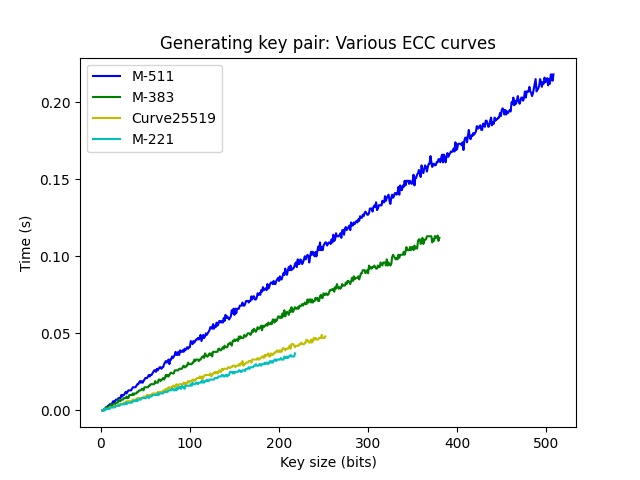
\includegraphics[width=\linewidth]{figures/Timing.png}
        \caption{Some curves faster than others}
        \label{fig:curves}
    \end{minipage}
\end{figure}

\vspace{5mm}

After demonstrating the benefits of ECC over RSA, the focus then shifts to the benefits of some ECC curves over others. 

Figure \ref{fig:curves} shows how the time taken to generate a key pair varies as the size of the private key increases, for 4 different curves. 
This, as before, means timing the operations of selecting a private key $k$ of a given size and then generating the corresponding public key $kG$ by 
multiplying the curve's base point $G$ by this number. 

The key finding from Figure \ref{fig:curves} is that, while the time taken by every curve increases linearly, 
the speed of this increase (the gradient of the line) is greater for some curves than others. 
These differences can be explained by the properties of each curve. 
Recall from Section \ref{Elliptic Curve} that an elliptic curve is defined over a finite field modulo $p$. 
This means that if the calculation of a coordinate produces a result greater than $p$, $p$ is subtracted from this result to produce a much smaller number. 
Therefore no point can have an x or y-coordinate greater than $p$. 
If a curve is defined to have a larger $p$, the points on the curve can have larger coordinates, 
so calculations involving these points will take longer. 
This explains the differences in gradients of the 4 lines in Figure \ref{fig:curves}, 
since curve M-221 has $p \approx 2^{221}$ while curve M-511 has $p \approx 2^{511}$. 

Another point to note about Figure \ref{fig:curves} is that some lines on the graph are shorter than others. 
This is due to another property of each curve. 
Recall from Section \ref{SharedKey} that the base point $G$ of every curve has an order $n$, where $nG=0$. 
What this means in practice, as mentioned in Section \ref{SharedKey}, 
is that the private keys used with a given curve must be less than $n$. 
When it came to producing the results in Figure \ref{fig:curves}, the key sizes for each curve could only range from $1$ to $n$, 
and $n$ is different for every curve. 
For example, the order of curve M-221's base point is $n \approx 2^{218}$, while curve M-511's is $n \approx 2^{508}$. 
This explains the length of each line in Figure \ref{fig:curves}, the line for M-221 ends at 218 bits and the line for M-511 ends at 508 bits. 

The minimum recommended security requirements for ECC key size today is 224 bits \cite[p54-55]{barker2020recommendation}. 
This means that curve M-221 is not considered secure anymore, but the other three curves are secure since their $n < 2^{224}$. 
This minimum requirement for key size will increase in the future as computers get faster. 
Therefore, while Curve25519 is today's fastest secure curve, 
curves M-383 and M-511 will still be considered secure further into the future. 


\subsection{Security} \noindent \label{Security}
This subsection analyses my system for security vulnerabilities, 
specifically whether my implementation leaks any secret data through side-channel attacks such as timing attacks. 
If there is a correlation between the properties of a secret value and the time taken by an operation involving this value, 
an attacker could use a timing attack to gain some information about the supposedly secret value. 
In terms of my system, the secret value is the private key $k$ and the operation is the calculation of the public key $kG$, 
in which the base point $G$ is multiplied by the private key $k$. 
This operation is carried out by repeated doubling and adding of the base point $G$, until reaching $kG$. 
If an attacker is able to isolate and time this operation, knowing that there was a correlation, 
they could infer information about the private key from measuring how long the operation took. 
To check if my system leaked side-channel information in this way, 
I used the system to generate 300 random key pairs, timing the time taken by the process each time. 
I plotted these times against two different properties of the private key: 
the number of $1$ bits in the binary expansion of the key (Figure \ref{fig:number1s}), 
and the size of the key, measured by taking the log of the key (Figure \ref{fig:logkey}). 

\begin{figure}[!htb]
    \begin{minipage}{0.5\textwidth}
        \centering
        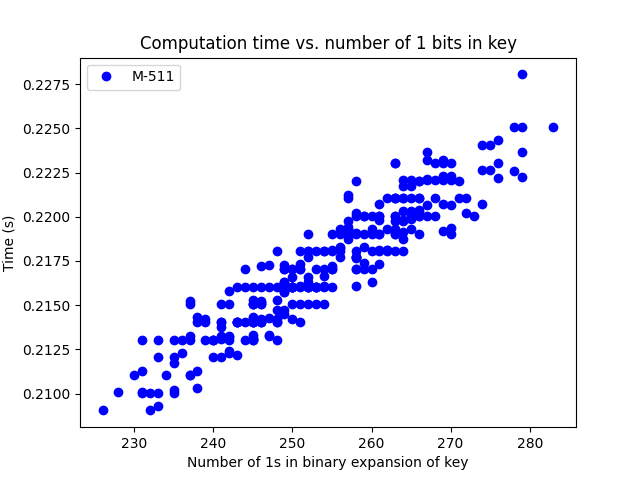
\includegraphics[width=\linewidth]{figures/1bits.png}
        \caption{Correlation with number of 1s in key}
        \label{fig:number1s}
    \end{minipage}\hfill
    \begin{minipage}{0.5\textwidth}
        \centering
        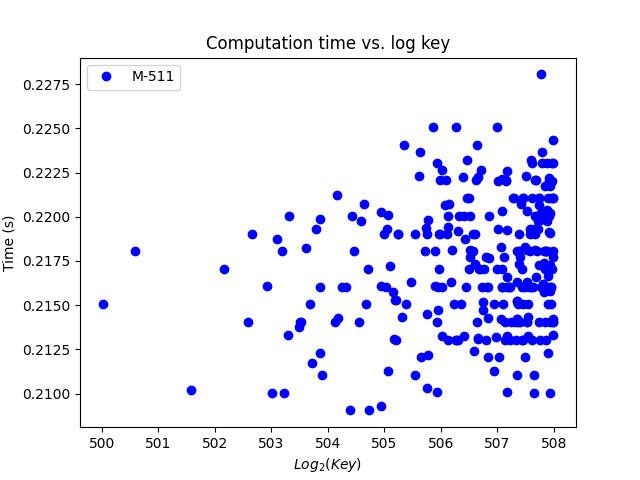
\includegraphics[width=\linewidth]{figures/logKey.png}
        \caption{No strong correlation with key size}
        \label{fig:logkey}
    \end{minipage}
\end{figure}

Figure \ref{fig:number1s} appears to show a positive correlation between the number of 1s in the binary expansion of the private key and the time taken to generate the key pair. 
However, Figure \ref{fig:logkey} appears to show no strong correlation between the value of the private key and the time taken to generate the key pair. 

The correlation shown in Figure \ref{fig:number1s} can be explained by examining the doubling and adding procedure. 
To simplify, the system doubles the point $G$ repeatedly to produce $2G$, $4G$, ..., $2^{log_2(k)} \cdot G$. 
Then, the relevant doublings are each added to produce the result, 
so if the $i^{th}$ bit in the binary expansion of $k$ is a $1$, $2^i \cdot G$ is added. 
%This is how the point multiplication of $kG$ is calculated in $O(log(k))$ running time. 
Therefore, the more $1$ bits there are in $k$, the more point additions will have to be done. 
Since every operation of point addition takes some amount of time, the total time taken will increase as the number of point additions increases. 
This is why Figure \ref{fig:number1s} shows a positive correlation. 

The lack of strong correlation shown in Figure \ref{fig:logkey} can be explained by considering the scale of the axis in comparison to that of 
Figure \ref{fig:curves}. 
Figure \ref{fig:curves} shows that there is a strong positive correlation between private key size and time taken to generate a key pair, 
but that is over the entire range of key sizes 0 to 508. 
Since here in Figure \ref{fig:logkey} the private key is randomly chosen from the range $[1-n]$ where $n \approx 2^{508}$, 
the most common key size is 508 bits ($2^{507}-2^{508}$), with half as many keys for every bit decrease. 
This explains both why the spread of points in Figure \ref{fig:logkey} is so concentrated on the right side, 
and why the number of points in each interval approximately halves moving from left to right. 
This is representative of how the system performs in practice. 
The relatively small variation in both axes of Figure \ref{fig:logkey} means that random error (noise or natural variation) 
plays a much more significant role in the timing results and obscures the underlying positive correlation between key size and time taken. 
Therefore, my system does not show a strong correlation between the key size and the time taken in practice. 


\section{Evaluation} \noindent
This section should between 1 to 2 pages in length.

- 20\% of paper

- Suitability of approach

- Discussion of strengths and limitations of the system - limitations with communicating over networks, works well with multiple client instances on a local machine

- Discussion of algorithms used - ECDH, ECDSA, point addition and point multiplication

- Appraisal of project organisation

A possible solution to the issue shown in Figure \ref{fig:number1s} is to add a timing delay to the system such that the key pair generation always takes the same amount of time. 
The system would generate the key pair and then wait until a given time had elapsed before returned the result, 
meaning that an attacker could not infer any information about the private key. 


\section{Conclusions} \noindent
This section summarises the main points of this paper. 
Do not replicate the abstract as the conclusion. 
A conclusion might elaborate on the importance of the work or suggest applications and extensions. 
This section should be no more than 1 page in length. 

- 5\% of paper

- Description of the main findings

- Clarity of conclusions

- Discussion of further work

Much research has been done into Elliptic Curve Cryptography since its discovery in 1985 \cite{10.1007/3-540-39799-X_31,koblitz1987elliptic}. 
The security of ECC is based on the hardness of the ECDLP, 
and currently the best algorithms known to solve the ECDLP have fully exponential running time. 
In contrast to the subexponential-time algorithms known for the integer factorisation problem, 
on which the security of RSA is based. 
This means that, for example, a 160-bit EC key provides the same level of security as a 1024-bit RSA key \cite{hankerson2003guide,silverman2009arithmetic}. 
ECC is a very strong encryption method, but only when implemented properly, 
using a safe curve \cite{bernstein2013safecurves,10.1007/11745853_14}
and a good random number generator \cite{hotz2010console}. 


\bibliography{projectpaper}


\end{document}
